%\section{Racine d'un polynôme du second degré}

%\subsection{Discriminant et racine}
\def\rdifficulty{1}
\begin{EXO}{Calcul de discriminants}{}
Pour chaque trinôme ci-dessous, calculer le discriminant $\Delta$
\begin{tcbenumerate}[4]
%\begin{tabular}{p{4cm}p{4cm}p{4cm}p{4cm}}
\tcbitem \tcbitempoint{1} $x^2+4x+5$
\tcbitem \tcbitempoint{1} $2x^2-x-6$
\tcbitem \tcbitempoint{1} $-2x^2-4x-7$
\tcbitem \tcbitempoint{1} $-x^2+2x+3$ \\
%\end{tabular}
\end{tcbenumerate}

\exocorrection

\begin{tcbenumerate}[2]
\tcbitem Pour $x^2+4x+5$ :

On a $a=1$, $b=4$ et $c=5$

$\Delta = b^2-4ac = 4^2-4\times1\times5 = 16-20 = -4$

\tcbitem Pour $2x^2-x-6$ :

On a $a=2$, $b=-1$ et $c=-6$

$\Delta = b^2-4ac = (-1)^2-4\times2\times(-6) = 1+48 = 49$

\tcbitem Pour $-2x^2-4x-7$ :

On a $a=-2$, $b=-4$ et $c=-7$

$\Delta = b^2-4ac = (-4)^2-4\times(-2)\times(-7) = 16-56 = -40$

\tcbitem Pour $-x^2+2x+3$ :

On a $a=-1$, $b=2$ et $c=3$

$\Delta = b^2-4ac = 2^2-4\times(-1)\times3 = 4+12 = 16$
\end{tcbenumerate}
\end{EXO}

\vspace{-1mm}
\def\rdifficulty{1}
\begin{EXO}{Nombre de solutions}{}
Déterminer le nombre de solutions réelles de chaque équation ci-dessous.
\begin{tcbenumerate}[4]
%\begin{tabular}{p{4cm}p{4cm}p{4cm}p{4cm}}
\tcbitem \tcbitempoint{1} $x^2+3x+2=0$
\tcbitem \tcbitempoint{1} $2x^2-5x+7=0$
\tcbitem \tcbitempoint{1} $-\dfrac{1}{3}x^2+2x-3=0$
\tcbitem \tcbitempoint{1} $2x^2+7x+11=0$ \\
%\end{tabular}
\end{tcbenumerate}

\exocorrection

\begin{tcbenumerate}[1]
\tcbitem Pour $x^2+3x+2=0$ :

\nombresolutions{1}{3}{2}

\tcbitem Pour $2x^2-5x+7=0$ :

\nombresolutions{2}{-5}{7}

\tcbitem Pour $-\dfrac{1}{3}x^2+2x-3=0$ :

\nombresolutions{-0.333333}{2}{-3}

\tcbitem Pour $2x^2+7x+11=0$ :

\nombresolutions{2}{7}{11}
\end{tcbenumerate}
\end{EXO}

\vspace{-1mm}
\def\rdifficulty{1.5}
\begin{EXO}{Signe du discriminant}{}
Pour chaque fonction représentée ci dessous, déterminer le signe de $\Delta$.

\noindent \begin{minipage}{4cm}
\tikzinclude{TnVi}
\end{minipage}
\hspace{3mm}
\begin{minipage}{4cm}
\tikzinclude{XWyE}
\end{minipage}
\hspace{3mm}
\begin{minipage}{4cm}
\tikzinclude{bxUA}
\end{minipage}
\hspace{3mm}
\begin{minipage}{4cm}
\tikzinclude{zaPA}
\end{minipage}

\exocorrection

\begin{tcbenumerate}[1]
\tcbitem \textbf{Figure 1 :} La parabole coupe l'axe des abscisses en deux points distincts donc $\Delta > 0$

\tcbitem \textbf{Figure 2 :} La parabole est tangente à l'axe des abscisses (un seul point d'intersection) donc $\Delta = 0$

\tcbitem \textbf{Figure 3 :} La parabole ne coupe pas l'axe des abscisses donc $\Delta < 0$

\tcbitem \textbf{Figure 4 :} La parabole coupe l'axe des abscisses en deux points distincts donc $\Delta > 0$
\end{tcbenumerate}
\end{EXO}

\vspace{-1mm}
\def\rdifficulty{1.5}
\begin{EXO}{Résolution d'équations}{}
Résoudre dans $\R$ les équations suivantes
\begin{tcbenumerate}[3]
%\begin{tabular}{p{5cm}p{5cm}p{5cm}}
\tcbitem \tcbitempoint{1} $3x^2-9x-12=0$
\tcbitem \tcbitempoint{1} $2x^2+5x+7=0$
\tcbitem \tcbitempoint{1} $2x^2-2x+\dfrac{1}{2}=0$ \\
%\end{tabular}
\end{tcbenumerate}

\exocorrection

\begin{tcbenumerate}[1]
\tcbitem Pour $3x^2-9x-12=0$ :

\resoudreequation{3}{-9}{-12}{}

\tcbitem Pour $2x^2+5x+7=0$ :

\resoudreequation{2}{5}{7}{}

\tcbitem Pour $2x^2-2x+\dfrac{1}{2}=0$ :

\resoudreequation{2}{-2}{0.5}{}
\end{tcbenumerate}
\end{EXO}

\vspace{-1mm}
\def\rdifficulty{1.5}
\begin{EXO}{Racines de trinômes}{}
Déterminer, si elles existent, les racines des trinômes suivants :
\begin{tcbenumerate}[3]
%\begin{tabular}{p{5cm}p{5cm}p{5cm}}
\tcbitem \tcbitempoint{1} $f(x)=-2x^2+3x-4$
\tcbitem \tcbitempoint{1} $g(x)=\dfrac{1}{2}x^2-4x+8$
\tcbitem \tcbitempoint{1} $h(x)=-x^2-2x+35$ \\
%\end{tabular}
\end{tcbenumerate}

\exocorrection

\begin{tcbenumerate}[1]
\tcbitem Pour $f(x)=-2x^2+3x-4$ :

\resoudreequation{-2}{3}{-4}{}

\tcbitem Pour $g(x)=\dfrac{1}{2}x^2-4x+8$ :

\resoudreequation{0.5}{-4}{8}{}

\tcbitem Pour $h(x)=-x^2-2x+35$ :

\resoudreequation{-1}{-2}{35}{}
\end{tcbenumerate}
\end{EXO}

\vspace{-1mm}
\def\rdifficulty{2}
\begin{EXO}{Nombres consécutifs}{}
Déterminer deux nombres entiers consécutifs dont la somme des carrés est égale à $4141$

\exocorrection

\tcbitempoint{2} Soit $n$ le premier nombre, le suivant est $n+1$.

On a donc : $n^2 + (n+1)^2 = 4141$

$n^2 + n^2 + 2n + 1 = 4141$

$2n^2 + 2n + 1 = 4141$

$2n^2 + 2n - 4140 = 0$

On divise par 2 : $n^2 + n - 2070 = 0$

\resoudreequation{1}{1}{-2070}{}

On garde la solution positive : $n = 45$

Les deux nombres sont donc $45$ et $46$.

\textbf{Vérification :} $45^2 + 46^2 = 2025 + 2116 = 4141$ \checkmark
\end{EXO}

\vspace{-1mm}
\def\rdifficulty{2}
\begin{EXO}{Équations quotients}{}
Résoudre les équations suivantes :
\begin{tcbenumerate}[2]
%\begin{tabular}{p{4cm}p{4cm}}
\tcbitem \tcbitempoint{2} $\dfrac{5x^2-12,5x-7,5}{3-x}=0$
\tcbitem \tcbitempoint{2} $\dfrac{x+20}{10}=\dfrac{10}{x}$ \\
%\end{tabular}
\end{tcbenumerate}

\exocorrection

\begin{tcbenumerate}[1]
\tcbitem $\dfrac{5x^2-12,5x-7,5}{3-x}=0$

Une fraction est nulle si et seulement si son numérateur est nul et son dénominateur non nul.

Condition d'existence : $3-x \neq 0$ donc $x \neq 3$

On résout $5x^2-12,5x-7,5=0$ :

\resoudreequation{5}{-12.5}{-7.5}{}

Les solutions sont $3$ et $-0,5$. Mais $x=3$ est exclu, donc $S = \ensembleDiscret{-0,5}$

\tcbitem $\dfrac{x+20}{10}=\dfrac{10}{x}$

Condition d'existence : $x \neq 0$

On multiplie en croix : $x(x+20) = 10 \times 10$

$x^2 + 20x = 100$

$x^2 + 20x - 100 = 0$

\resoudreequation{1}{20}{-100}{}
\end{tcbenumerate}
\end{EXO}

\vspace{-1mm}
\def\rdifficulty{1.5}
\begin{EXO}{Programme de calcul}{}
On considère le programme de calcul ci-après :

\begin{tcbenumerate}[2]
\tcbitem \tcbitempoint{1} Si on choisit le nombre $5$, quel nombre obtient-on ?
\tcbitem \tcbitempoint{2} Pour quel nombre de départ obtient on $91$ ?
\end{tcbenumerate}
\exocorrection

\begin{tcbenumerate}[1]
\tcbitem Si $a=5$ : $b=5^2=25$, $c=25+2 \times 5 = 35$, $d=35-8=27$

On obtient \textbf{27}.

\tcbitem Le programme calcule : $a^2 + 2a - 8$

On cherche $a$ tel que $a^2 + 2a - 8 = 91$

$a^2 + 2a - 8 = 91$

$a^2 + 2a - 99 = 0$

\resoudreequation{1}{2}{-99}{}
\end{tcbenumerate}
\end{EXO}
\begin{CodePiton}{}
a=eval(input(("Choisir un nombre"))
b=a**2
c=b+2*a
d=c-8
print("Le resultat est ",d)
\end{CodePiton}


\def\rdifficulty{2}
\begin{EXO}{Somme et produit}{}
Trouver deux entiers dont la somme est égale à $40$ et le produit à $375$

\exocorrection

Soit $x$ et $y$ les deux nombres.

On a : $\begin{cases} x + y = 40 \\ xy = 375 \end{cases}$

De la première équation : $y = 40 - x$

En substituant dans la seconde : $x(40-x) = 375$

$40x - x^2 = 375$

$-x^2 + 40x - 375 = 0$ ou $x^2 - 40x + 375 = 0$

\resoudreequation{1}{-40}{375}{}

Les deux nombres sont $15$ et $25$.

\textbf{Vérification :} $15 + 25 = 40$ et $15 \times 25 = 375$ \checkmark
\end{EXO}

\vspace{-1mm}
\def\rdifficulty{2.5}
\begin{EXO}{Polygone et aires}{}
Soit ABCD un carré de coté $x cm$ et BEC un triangle isocèle en $E$ de hauteur $2 cm$.

On note $A(x)$ l'aire du polygone ABECD en $cm^2$.
\begin{tcbenumerate}[2]
\tcbitem \tcbitempoint{1} Faire un dessin représentant la situation.
\tcbitem \tcbitempoint{1} Quelles valeurs peut prendre $x$ ?
\tcbitem \tcbitempoint{1} Déterminer l'expression de $A(x)$ en fonction de $x$.
\tcbitem \tcbitempoint{1} Quelle est la valeur de $A(x)$ si $x$ est égal à $5$ ?
\tcbitem[raster multicolumn=2]  \tcbitempoint{2} Pour quelle(s) valeur(s) de $x$ a-t-on $A(x)=24,75$ ?
\end{tcbenumerate}

\exocorrection

\begin{tcbenumerate}[1]
    \tcbitem Il y a deux cas possibles : E est \acc{intérieur au carré}, ou E est \acc{extérieur au carré}.
    
    \bcattention Dans la suite de l'exercice, on traitera uniquement le cas avec E \acc{extérieur} au carré. 

    L'autre cas se traite de la même manière que le premier et la solution est fournie dans la seconde image pour auto-vérification.

    \begin{MultiColonnes}{2}[colframe=gray!75!black,coltitle=white,boxrule=0.4pt]
\tcbitem[halign=center,valign=center,title=Le cas avec E extérieur :]

\definecolor{ffqqqq}{rgb}{1.,0.,0.}
\definecolor{qqttcc}{rgb}{0.,0.2,0.8}
\definecolor{uuuuuu}{rgb}{0.26666666666666666,0.26666666666666666,0.26666666666666666}
\definecolor{ududff}{rgb}{0.30196078431372547,0.30196078431372547,1.}
\definecolor{uququq}{rgb}{0.25098039215686274,0.25098039215686274,0.25098039215686274}
\begin{tikzpicture}[line cap=round,line join=round,>=triangle 45,x=1.0cm,y=1.0cm]
\clip(-1.,-0.5) rectangle (7.5,7.5);
\fill[line width=1.2pt,color=qqttcc,fill=qqttcc,fill opacity=0.10000000149011612] (0.,0.) -- (4.5,0.) -- (6.5,2.25) -- (4.5,4.5) -- (0.,4.5) -- cycle;
\draw[line width=4.pt,color=uququq] (5.029331392810919,9.79446157067848) -- (8.623629108433676,9.79446157067848);
\draw [line width=1.2pt,color=qqttcc] (0.,0.)-- (4.5,0.);
\draw [line width=1.2pt,color=qqttcc] (4.5,0.)-- (6.5,2.25);
\draw [line width=1.2pt,color=qqttcc] (6.5,2.25)-- (4.5,4.5);
\draw [line width=1.2pt,color=qqttcc] (4.5,4.5)-- (0.,4.5);
\draw [line width=1.2pt,color=qqttcc] (0.,4.5)-- (0.,0.);
\draw [line width=1.2pt,dash pattern=on 2pt off 2pt] (4.5,4.5)-- (4.5,0.);
\draw [line width=1.2pt,color=ffqqqq] (4.5,2.25)-- (6.5,2.25);
\draw (-0.416029646357559,6.32596427510252) node[anchor=north west] {$\color{blue}\large \text{Aire}_{ABE_1CD} = \num{24.75} \,\text{cm}^2$};
\draw (-0.43400113493567277,7.22453870400821) node[anchor=north west] {$\large x = \num{4.5}\,\text{cm}$};
%\begin{scriptsize}
\draw [color=uququq] (5.8380483788260396,9.79446157067848)-- ++(-2.5pt,0 pt) -- ++(5.0pt,0 pt) ++(-2.5pt,-2.5pt) -- ++(0 pt,5.0pt);
\draw[color=uququq] (6.017763264607177,10.216791552264155) node {$a = 4.5$};
\draw [color=ududff] (0.,0.)-- ++(-3.0pt,0 pt) -- ++(6.0pt,0 pt) ++(-3.0pt,-3.0pt) -- ++(0 pt,6.0pt);
\draw[color=ududff] (-0.6137160207168106,0.2605868799891171) node {$A$};
\draw [color=uuuuuu] (4.5,0.)-- ++(-3.0pt,0 pt) -- ++(6.0pt,0 pt) ++(-3.0pt,-3.0pt) -- ++(0 pt,6.0pt);
\draw[color=uuuuuu] (5.173103301435829,0.1168149713642068) node {$B$};
\draw [color=uuuuuu] (4.5,4.5)-- ++(-3.0pt,0 pt) -- ++(6.0pt,0 pt) ++(-3.0pt,-3.0pt) -- ++(0 pt,6.0pt);
\draw[color=uuuuuu] (4.633958644092416,4.8612879559862465) node {$C$};
\draw [color=uuuuuu] (0.,4.5)-- ++(-3.0pt,0 pt) -- ++(6.0pt,0 pt) ++(-3.0pt,-3.0pt) -- ++(0 pt,6.0pt);
\draw[color=uuuuuu] (-0.45197262351378664,4.897230933142475) node {$D$};
\draw [color=uuuuuu] (4.5,2.25)-- ++(-3.0pt,0 pt) -- ++(6.0pt,0 pt) ++(-3.0pt,-3.0pt) -- ++(0 pt,6.0pt);
\draw[color=uuuuuu] (3.969013566702205,2.7406523037688197) node {$H$};
\draw [color=uuuuuu] (6.5,2.25)-- ++(-3.0pt,0 pt) -- ++(6.0pt,0 pt) ++(-3.0pt,-3.0pt) -- ++(0 pt,6.0pt);
\draw[color=uuuuuu] (6.6737225977083305,2.6597806051673074) node {$E_1$};
\draw[color=ffqqqq] (5.155131812857715,2.7406523037688197) node {2cm};
%\end{scriptsize}
\end{tikzpicture}
    \tcbitem[title=Le cas avec E intérieur :,halign=center,valign=center]

    \definecolor{ttzzqq}{rgb}{0.2,0.6,0.}
\definecolor{ffqqqq}{rgb}{1.,0.,0.}
\definecolor{uuuuuu}{rgb}{0.26666666666666666,0.26666666666666666,0.26666666666666666}
\definecolor{ududff}{rgb}{0.30196078431372547,0.30196078431372547,1.}
\definecolor{uququq}{rgb}{0.25098039215686274,0.25098039215686274,0.25098039215686274}
\begin{tikzpicture}[line cap=round,line join=round,>=triangle 45,x=1.0cm,y=1.0cm]
\clip(-1.,-0.5) rectangle (7.5,8.5);
\fill[line width=1.2pt,color=ttzzqq,fill=ttzzqq,fill opacity=0.10000000149011612] (0.,0.) -- (5.5,0.) -- (3.5,2.75) -- (5.5,5.5) -- (0.,5.5) -- cycle;
\draw[line width=4.pt,color=uququq] (5.856019867404153,10.818836419630967) -- (9.45031758302691,10.818836419630967);
\draw [line width=1.2pt,dash pattern=on 3pt off 3pt] (5.5,5.5)-- (5.5,0.);
\draw (-0.20037178342019252,8.46457141589806) node[anchor=north west] {$\large x = \num{5.5}\,\text{cm}$};
\draw [line width=1.2pt,color=ffqqqq] (5.5,2.75)-- (3.5,2.75);
\draw [line width=1.2pt,color=ttzzqq] (0.,0.)-- (5.5,0.);
\draw [line width=1.2pt,color=ttzzqq] (5.5,0.)-- (3.5,2.75);
\draw [line width=1.2pt,color=ttzzqq] (3.5,2.75)-- (5.5,5.5);
\draw [line width=1.2pt,color=ttzzqq] (5.5,5.5)-- (0.,5.5);
\draw [line width=1.2pt,color=ttzzqq] (0.,5.5)-- (0.,0.);
\draw (-0.3621151806232166,7.548025498414257) node[anchor=north west] {$\color{red}\large \text{Aire}_{ABE_2CD} =  \num{24.75} \,\text{cm}^2$};
%\begin{scriptsize}
\draw [color=uququq] (6.844451739200411,10.818836419630967)-- ++(-2.5pt,0 pt) -- ++(5.0pt,0 pt) ++(-2.5pt,-2.5pt) -- ++(0 pt,5.0pt);
\draw[color=uququq] (6.9343091820909795,11.241166401216642) node {$a = \num{5.5}$};
\draw [color=ududff] (0.,0.)-- ++(-3.0pt,0 pt) -- ++(6.0pt,0 pt) ++(-3.0pt,-3.0pt) -- ++(0 pt,6.0pt);
\draw[color=ududff] (-0.6137160207168096,0.2605868799891171) node {$A$};
\draw [color=uuuuuu] (5.5,0.)-- ++(-3.0pt,0 pt) -- ++(6.0pt,0 pt) ++(-3.0pt,-3.0pt) -- ++(0 pt,6.0pt);
\draw[color=uuuuuu] (6.161535173232088,0.1168149713642068) node {$B$};
\draw [color=uuuuuu] (5.5,5.5)-- ++(-3.0pt,0 pt) -- ++(6.0pt,0 pt) ++(-3.0pt,-3.0pt) -- ++(0 pt,6.0pt);
\draw[color=uuuuuu] (5.622390515888674,5.867691316360619) node {$C$};
\draw [color=uuuuuu] (0.,5.5)-- ++(-3.0pt,0 pt) -- ++(6.0pt,0 pt) ++(-3.0pt,-3.0pt) -- ++(0 pt,6.0pt);
\draw[color=uuuuuu] (-0.45197262351378553,5.903634293516847) node {$D$};
\draw [color=uuuuuu] (5.5,2.75)-- ++(-3.0pt,0 pt) -- ++(6.0pt,0 pt) ++(-3.0pt,-3.0pt) -- ++(0 pt,6.0pt);
\draw[color=uuuuuu] (6.413136013325681,3.0821105867529814) node {$H$};
\draw [color=uuuuuu] (3.5,2.75)-- ++(-3.0pt,0 pt) -- ++(6.0pt,0 pt) ++(-3.0pt,-3.0pt) -- ++(0 pt,6.0pt);
\draw[color=uuuuuu] (2.9176814848825496,3.396611636869973) node {$E_2$};
\draw[color=ffqqqq] (4.41830078115505,3.2438539839560057) node {2 cm};
%\end{scriptsize}
\end{tikzpicture}
\end{MultiColonnes}

\tcbitem $x > 0$ (côté strictement positif)

\tcbitem $A(x) = \text{Aire carré} + \text{Aire triangle} = x^2 + \dfrac{x \times 2}{2} = x^2 + x$

\tcbitem $A(5) = 5^2 + 5 = 25 + 5 = 30$ cm$^2$

\tcbitem On résout $x^2 + x = 24,75$ :

$x^2 + x - 24,75 = 0$

\resoudreequation{1}{1}{-24.75}{}

Comme $x > 0$, on garde $x = 4,5$ cm.
\end{tcbenumerate}
\end{EXO}

\vspace{-1mm}
\def\rdifficulty{2.5}
\begin{EXO}{Équation paramétrique}{}
On considère l'équation $(m+8)x^2+mx+1=0$. Pour quelles valeurs de $m$ cette équation admet-elle une unique solution ?

\exocorrection

Une équation du second degré admet une unique solution si et seulement si son discriminant est nul.

On a : $a = m+8$, $b = m$, $c = 1$

\textbf{Discriminant de l'équation en $x$ (en fonction de $m$) :}

$\Delta_x = b^2 - 4ac = m^2 - 4(m+8)(1) = m^2 - 4m - 32$

On cherche $\Delta_x = 0$ :

$m^2 - 4m - 32 = 0$

\textbf{Résolution de l'équation en $m$ :}

\resoudreequation{1}{-4}{-32}{}

L'équation en $x$ admet une unique solution pour $m = -4$ ou $m = 8$.
\end{EXO}

\vspace{-1mm}
\def\rdifficulty{3}
\begin{EXO}{Équations degré 3}{}
\begin{tcbenumerate}[2]
\tcbitem[boxrule=0.4pt,colframe=black,raster multicolumn=2] Soit $f$ la fonction définie sur $\R$ par $f(x)=x^3-2x^2-5x+6$.

On veut résoudre l'équation $f(x)=0$.
\begin{tcbenumerate}[2][1][alph]
\tcbitem \tcbitempoint{0.5} Vérifier que $1$ est solution de l'équation $f(x)=0$.
\tcbitem \tcbitempoint{1} Montrer que l'on peut écrire $f(x)$ sous la forme $(x-1)(ax^2+bx+c)$ en développant et en identifiant les coefficients. On donnera les valeurs de $a$, $b$, et $c$.
\tcbitem \tcbitempoint{1} Résoudre l'équation $ax^2+bx+c=0$
\tcbitem \tcbitempoint{0.5} En déduire toutes les solutions de $f(x)=0$, et la forme factorisée de $f$.
\end{tcbenumerate}
\tcbitem[boxrule=0.4pt,colframe=black,raster multicolumn=2] On souhaite maintenant résoudre l'équation $2x^3-20x^2-618x+1980=0$.
\begin{tcbenumerate}[2][1][alph]
\tcbitem \tcbitempoint{1} Vérifier que $3$ est solution, puis écrire le premier terme de l'équation sous la forme $(x-3)\times g(x)$, avec $g(x)$ un polynôme de degré 2.
\tcbitem \tcbitempoint{1} En déduire toutes les solutions de l'équation.
\end{tcbenumerate}
\end{tcbenumerate}

\exocorrection

\begin{tcbenumerate}[1]
\tcbitem \textbf{Partie 1 :}
\begin{tcbenumerate}[1][1][alph]
\tcbitem $f(1) = 1^3 - 2(1)^2 - 5(1) + 6 = 1 - 2 - 5 + 6 = 0$ \checkmark

\tcbitem On développe $(x-1)(ax^2+bx+c) = ax^3 + bx^2 + cx - ax^2 - bx - c = ax^3 + (b-a)x^2 + (c-b)x - c$

Par identification avec $x^3-2x^2-5x+6$ :
\begin{itemize}
\item Coefficient de $x^3$ : $a = 1$
\item Coefficient de $x^2$ : $b-a = -2$ donc $b = -2+1 = -1$
\item Coefficient de $x$ : $c-b = -5$ donc $c = -5-1 = -6$
\item Terme constant : $-c = 6$ donc $c = -6$ \checkmark
\end{itemize}

Donc $a=1$, $b=-1$, $c=-6$

\tcbitem On résout $x^2-x-6=0$ :

\resoudreequation{1}{-1}{-6}{}

\tcbitem Les solutions de $f(x)=0$ sont $x=1$, $x=-2$ et $x=3$

Forme factorisée : $f(x) = (x-1)(x+2)(x-3)$
\end{tcbenumerate}

\tcbitem \textbf{Partie 2 :}
\begin{tcbenumerate}[1][1][alph]
\tcbitem $2(3)^3-20(3)^2-618(3)+1980 = 54-180-1854+1980 = 0$ \checkmark

Par division euclidienne ou identification : $2x^3-20x^2-618x+1980 = (x-3)(2x^2-14x-660)$

\tcbitem On résout $2x^2-14x-660=0$ ou $x^2-7x-330=0$ :

\resoudreequation{1}{-7}{-330}{}

Les solutions sont $x=3$, $x=-15$ et $x=22$
\end{tcbenumerate}
\end{tcbenumerate}
\end{EXO}

%\subsection{Propriétés des racines}

\vspace{-3mm}
\def\rdifficulty{1.5}
\begin{EXO}{Somme et produit de racines}{}
Soit $f$ la fonction définie sur $\R$ par $f(x)=2x^2-5x+1$.
\begin{tcbenumerate}[2]
\tcbitem \tcbitempoint{1} Calculer le discriminant $\Delta$.
\tcbitem \tcbitempoint{1} Vérifier que $\Delta >0$, et en déduire le nombre de racines de $f$.
\tcbitem[raster multicolumn=2] \tcbitempoint{1} Sans calculer les racines, déterminer leur somme et leur produit.
\end{tcbenumerate}

\exocorrection

\begin{tcbenumerate}[1]
\tcbitem \calculerdiscriminant{2}{-5}{1}

\tcbitem On a $\Delta = 17 > 0$, donc $f$ admet deux racines réelles distinctes.

\tcbitem D'après les formules de Viète :

Somme des racines : $S = -\dfrac{b}{a} = -\dfrac{-5}{2} = \dfrac{5}{2}$

Produit des racines : $P = \dfrac{c}{a} = \dfrac{1}{2}$
\end{tcbenumerate}
\end{EXO}

\vspace{-1mm}
\def\rdifficulty{2}
\begin{EXO}{Trouver une racine}{}
Soit $f$ la fonction définie sur $\R$ par $f(x)=5x^2-4x-1$.
\begin{tcbenumerate}[2]
\tcbitem \tcbitempoint{1} Combien de racines $f$ admet-elle ?
\tcbitem \tcbitempoint{0.5} Vérifier que $f(1)=0$.
\tcbitem[raster multicolumn=2] \tcbitempoint{2} En utilisant la somme ou le produit des racines, trouver toutes les solutions de l'équation $f(x)=0$.
\end{tcbenumerate}

\exocorrection

\begin{tcbenumerate}[1]
\tcbitem \nombresolutions{5}{-4}{-1}

\tcbitem $f(1) = 5(1)^2 - 4(1) - 1 = 5 - 4 - 1 = 0$ \checkmark

\tcbitem Notons $x_1 = 1$ et $x_2$ l'autre racine.

\textbf{Méthode 1 (produit) :} $x_1 \times x_2 = \dfrac{c}{a} = \dfrac{-1}{5}$

Donc $1 \times x_2 = -\dfrac{1}{5}$ d'où $x_2 = -\dfrac{1}{5}$

\textbf{Méthode 2 (somme) :} $x_1 + x_2 = -\dfrac{b}{a} = -\dfrac{-4}{5} = \dfrac{4}{5}$

Donc $1 + x_2 = \dfrac{4}{5}$ d'où $x_2 = \dfrac{4}{5} - 1 = -\dfrac{1}{5}$

Les solutions sont $S = \ensembleDiscret{-\dfrac{1}{5} ; 1}$
\end{tcbenumerate}
\end{EXO}

\vspace{-1mm}
%\subsection{Résolution d'inéquations et signes}

\vspace{-3mm}
\def\rdifficulty{2}
\begin{EXO}{Tableaux de signes}{}
Dresser le tableau de signes de chaque fonction définie ci-dessous.
\vspace{-2mm}
\begin{tcbenumerate}[3]
%\begin{tabular}{p{5cm}p{5cm}p{5cm}}
\tcbitem \tcbitempoint{2} $f(x)=2x^2-4x-16$.
\tcbitem \tcbitempoint{2} $g(x)=9x^2+24x+16$.
\tcbitem \tcbitempoint{2} $h(x)=2x^2-5x+6$.\\
%\end{tabular}
\end{tcbenumerate}

\exocorrection

\begin{tcbenumerate}[1]
\tcbitem Pour $f(x)=2x^2-4x-16$ :

\seta{2}\setb{-4}\setc{-16}
\calculerdiscriminant{2}{-4}{-16}

$\Delta = 144 > 0$ donc deux racines :

\calculerracines{2}{-4}{-16}

Tableau de signes :

\tableausigne{2}{-4}{-16}

\tcbitem Pour $g(x)=9x^2+24x+16$ :

\calculerdiscriminant{9}{24}{16}

$\Delta = 0$ donc une racine double :

\calculerracines{9}{24}{16}

Tableau de signes :

\tableausigne{9}{24}{16}

\tcbitem Pour $h(x)=2x^2-5x+6$ :

\calculerdiscriminant{2}{-5}{6}

$\Delta = -23 < 0$ donc pas de racine réelle.

Le trinôme est toujours du signe de $a=2>0$, donc toujours positif.

Tableau de signes :

\tableausigne{2}{-5}{6}
\end{tcbenumerate}
\end{EXO}

\vspace{-2mm}
\def\rdifficulty{2}
\begin{EXO}{Inéquations du second degré}{}
Résoudre dans $\R$ les inéquations suivantes.
\vspace{-2mm}
\begin{tcbenumerate}[4]
%\begin{tabular}{p{4cm}p{4cm}p{4cm}p{4cm}}
\tcbitem \tcbitempoint{2} $5x^2-50,5x+5<0$
\tcbitem \tcbitempoint{1} $x^2+x+1>0$
\tcbitem \tcbitempoint{2} $3x^2-4x+\dfrac{4}{3}\leqslant 0$
\tcbitem \tcbitempoint{1} $-2x^2+3x-6<0$\\
%\end{tabular}
\end{tcbenumerate}

\exocorrection

\begin{tcbenumerate}[1]
\tcbitem Pour $5x^2-50,5x+5<0$ :

On a $a=5$, $b=-50{,}5$, $c=5$

$\Delta = b^2-4ac = (-50{,}5)^2-4\times5\times5 = 2550{,}25-100 = 2450{,}25 > 0$

Donc deux racines : $x_1 = \dfrac{50{,}5-\sqrt{2450{,}25}}{10} = 0{,}1$ et $x_2 = \dfrac{50{,}5+\sqrt{2450{,}25}}{10} = 10$

Tableau de signes : $a=5>0$, donc $f$ négative entre les racines.

$S = \CrochetG 0{,}1 ; 10 \CrochetG$

\tcbitem Pour $x^2+x+1>0$ :

On a $a=1$, $b=1$, $c=1$

$\Delta = 1^2-4\times1\times1 = 1-4 = -3 < 0$

Pas de racine réelle. Comme $a=1>0$, le trinôme est toujours positif.

$S = \R$

\tcbitem Pour $3x^2-4x+\dfrac{4}{3}\leqslant 0$ :

On a $a=3$, $b=-4$ et $c=\dfrac{4}{3}$

$\Delta = b^2-4ac = (-4)^2-4\times3\times\dfrac{4}{3} = 16-16 = 0$

Donc le trinôme admet une racine double :

$x_0 = \dfrac{-b}{2a} = \dfrac{4}{2\times3} = \dfrac{4}{6} = \dfrac{2}{3}$

Comme $a>0$ et $\Delta=0$, le trinôme est positif ou nul, et s'annule uniquement en $x_0=\dfrac{2}{3}$.

L'inéquation $3x^2-4x+\dfrac{4}{3}\leqslant 0$ n'est vérifiée que pour $x=\dfrac{2}{3}$.

$S = \ensembleDiscret{\dfrac{2}{3}}$

\tcbitem Pour $-2x^2+3x-6<0$ :

On a $a=-2$, $b=3$, $c=-6$

$\Delta = 3^2-4\times(-2)\times(-6) = 9-48 = -39 < 0$

Pas de racine réelle. Comme $a=-2<0$, le trinôme est toujours négatif.

$S = \R$
\end{tcbenumerate}
\end{EXO}

\vspace{-4mm}
%\subsection{Problèmes}

\vspace{-3mm}
\def\rdifficulty{2.5}
\begin{EXO}{Bénéfice d'entreprise}{}
Une entreprise produit entre $0$ et $50$ balançoires par jour.

Le coût de fabrication de $x$ balançoires, en euros, est donné par la fonction suivante : $f(x)=x^2+230x+325$

Chaque balançoire est vendue $300$\euro, et toute la production est vendue.

\begin{tcbenumerate}[2]
\tcbitem \tcbitempoint{1} Exprimer le bénéfice $B(x)$ réalisé par l'entreprise en fonction de $x$.
\tcbitem \tcbitempoint{1} Étudier les variations de la fonction $B$.
\tcbitem \tcbitempoint{1} En déduire le bénéfice maximal réalisé par l'entreprise.
\tcbitem \tcbitempoint{2} Combien de balançoires l'entreprise doit-elle produire et vendre pour être rentable ?
\end{tcbenumerate}

\exocorrection

\begin{tcbenumerate}[1]
\tcbitem Bénéfice = Recettes - Coûts

$B(x) = 300x - (x^2+230x+325) = 300x - x^2 - 230x - 325 = -x^2 + 70x - 325$

\tcbitem Forme canonique : $B(x) = -x^2 + 70x - 325 = -(x^2 - 70x) - 325$

$= -(x^2 - 70x + 35^2 - 35^2) - 325 = -(x-35)^2 + 1225 - 325 = -(x-35)^2 + 900$

Le sommet est en $(35; 900)$. Comme $a = -1 < 0$, la parabole est tournée vers le bas.

$B$ est croissante sur $[0;35]$ et décroissante sur $[35;50]$.

\tcbitem Le bénéfice maximal est atteint pour $x = 35$ balançoires, et vaut $900$\euro.

\tcbitem On cherche $B(x) \geq 0$ :

$-x^2 + 70x - 325 \geq 0$ ou $x^2 - 70x + 325 \leq 0$

\resoudreinequation{1}{-70}{325}{leq}
\end{tcbenumerate}
\end{EXO}

\def\rdifficulty{2}
\begin{EXO}{Formes factorisées}{}
Pour chaque trinôme ci-dessous, déterminer, si elle existe, sa forme factorisée :
\begin{tcbenumerate}[4]
%\begin{tabular}{p{4cm}p{4cm}p{4cm}p{4cm}}
\tcbitem \tcbitempoint{1.5} $f(x)=-\dfrac{1}{2}x^2+5x-12,5$
\tcbitem \tcbitempoint{1.5} $g(x)=4x^2+4x-8$
\tcbitem \tcbitempoint{1.5} $h(x)=2x^2-5x+6$
\tcbitem \tcbitempoint{1.5} $i(x)=3x^2-2x+2,4$\\
%\end{tabular}
\end{tcbenumerate}

\exocorrection

\begin{tcbenumerate}[1]
\tcbitem Pour $f(x)=-\dfrac{1}{2}x^2+5x-12,5$ :

\seta{-0.5}\setb{5}\setc{-12.5}
\calculerdiscriminant{-0.5}{5}{-12.5}

$\Delta = 0$ donc $f$ admet une racine double : \calculerracines{-0.5}{5}{-12.5}

Forme factorisée : $f(x) = -\dfrac{1}{2}(x-5)^2$

\tcbitem Pour $g(x)=4x^2+4x-8$ :

\resoudreequation{4}{4}{-8}{}

Forme factorisée : $g(x) = 4(x+2)(x-1)$

\tcbitem Pour $h(x)=2x^2-5x+6$ :

\calculerdiscriminant{2}{-5}{6}

$\Delta = -23 < 0$ donc $h$ n'admet pas de forme factorisée dans $\R$.

\tcbitem Pour $i(x)=3x^2-2x+2,4$ :

\calculerdiscriminant{3}{-2}{2.4}

$\Delta = -24,8 < 0$ donc $i$ n'admet pas de forme factorisée dans $\R$.
\end{tcbenumerate}
\end{EXO}

\def\rdifficulty{1.5}
\begin{EXO}{Identité remarquable}{}
Soit $f$ la fonction définie sur $\R$ par $f(x)=4(x-1)^2-16$.
\begin{tcbenumerate}[2]
\tcbitem \tcbitempoint{1} Écrire $f(x)$ sous la forme $a^2-b^2$
\tcbitem \tcbitempoint{1} En utilisant une identité remarquable, en déduire la forme factorisée de $f$.
\end{tcbenumerate}

\exocorrection

\begin{tcbenumerate}[1]
\tcbitem $f(x) = 4(x-1)^2 - 16 = [2(x-1)]^2 - 4^2$

Donc $f(x) = [2(x-1)]^2 - 4^2$ avec $a = 2(x-1)$ et $b = 4$

\tcbitem En utilisant $a^2-b^2 = (a-b)(a+b)$ :

$f(x) = [2(x-1) - 4][2(x-1) + 4]$

$= [2x-2-4][2x-2+4]$

$= (2x-6)(2x+2)$

$= 2(x-3) \times 2(x+1)$

$= 4(x-3)(x+1)$
\end{tcbenumerate}
\end{EXO}

\def\rdifficulty{3}
\begin{EXO}{Formes et équations}{}
Soit $f$ la fonction définie sur $\R$ par $f(x)=x^2-6x-27$
\begin{tcbenumerate}[2]
\tcbitem \tcbitempoint{1} Déterminer la forme canonique de $f$, en utilisant les identités remarquables.
\tcbitem \tcbitempoint{1} Déterminer la forme factorisée de $f$, en utilisant les identités remarquables.
\tcbitem[boxrule=0.4pt,colframe=black,raster multicolumn=2] En utilisant la forme adaptée, résoudre :
\vspace{-2mm}
\begin{tcbenumerate}[3][1][alph]
%\begin{tabular}{p{5cm}p{5cm}p{5cm}}
\tcbitem \tcbitempoint{0.5} $f(x)=0$
\tcbitem \tcbitempoint{1} $f(x)=-27$
\tcbitem \tcbitempoint{1} $f(x)=-36$\\
%\end{tabular}
\end{tcbenumerate}
\tcbitem[boxrule=0.4pt,colframe=black,raster multicolumn=2] Soit $g$ le fonction définie sur $\R$ par $g(x)=2x^2-\dfrac{3}{2}x-\dfrac{1}{2}$.
\begin{tcbenumerate}[2][1][alph]
\tcbitem \tcbitempoint{0.5} Vérifier que $1$ est racine de $g$.
\tcbitem \tcbitempoint{1} En utilisant la somme et le produit des racines, déterminer la valeur de l'autre racine de $g$.
\end{tcbenumerate}
\tcbitem \tcbitempoint{2} Résoudre $f(x)<g(x)$
\end{tcbenumerate}

\exocorrection

\begin{tcbenumerate}[1]
\tcbitem Forme canonique :

$f(x) = x^2 - 6x - 27 = (x^2 - 6x) - 27$

$= (x^2 - 6x + 9 - 9) - 27$

$= (x-3)^2 - 9 - 27$

$= (x-3)^2 - 36$

\tcbitem Forme factorisée (à partir de la canonique) :

$f(x) = (x-3)^2 - 36 = (x-3)^2 - 6^2$

$= [(x-3) - 6][(x-3) + 6]$

$= (x-9)(x+3)$

\tcbitem Résolutions :
\begin{tcbenumerate}[1][1][alph]
\tcbitem $f(x)=0$ : avec la forme factorisée

$(x-9)(x+3) = 0$ donc $x = 9$ ou $x = -3$

$S = \ensembleDiscret{-3 ; 9}$

\tcbitem $f(x)=-27$ : avec la forme canonique

$(x-3)^2 - 36 = -27$

$(x-3)^2 = 9$

$x-3 = 3$ ou $x-3 = -3$

$x = 6$ ou $x = 0$

$S = \ensembleDiscret{0 ; 6}$

\tcbitem $f(x)=-36$ : avec la forme canonique

$(x-3)^2 - 36 = -36$

$(x-3)^2 = 0$

$x = 3$

$S = \ensembleDiscret{3}$
\end{tcbenumerate}

\tcbitem Fonction $g$ :
\begin{tcbenumerate}[1][1][alph]
\tcbitem $g(1) = 2(1)^2 - \dfrac{3}{2}(1) - \dfrac{1}{2} = 2 - \dfrac{3}{2} - \dfrac{1}{2} = 2 - 2 = 0$ \checkmark

\tcbitem Soit $x_2$ l'autre racine. On utilise le produit :

$1 \times x_2 = \dfrac{c}{a} = \dfrac{-\frac{1}{2}}{2} = -\dfrac{1}{4}$

Donc $x_2 = -\dfrac{1}{4}$
\end{tcbenumerate}

\tcbitem Résoudre $f(x)<g(x)$ :

$x^2 - 6x - 27 < 2x^2 - \dfrac{3}{2}x - \dfrac{1}{2}$

$0 < x^2 + \dfrac{9}{2}x + \dfrac{53}{2}$ ou $x^2 + \dfrac{9}{2}x + \dfrac{53}{2} > 0$

On a $a=1$, $b=\dfrac{9}{2}$ et $c=\dfrac{53}{2}$

$\Delta = b^2-4ac = \left(\dfrac{9}{2}\right)^2-4\times1\times\dfrac{53}{2} = \dfrac{81}{4}-\dfrac{212}{4} = \dfrac{-131}{4} < 0$

Comme $a=1>0$ et $\Delta<0$, le trinôme est strictement positif pour tout $x\in\R$.

Donc l'inéquation $x^2 + \dfrac{9}{2}x + \dfrac{53}{2} > 0$ est toujours vraie.

$S = \R$
\end{tcbenumerate}
\end{EXO}

%\section*{Signe d'une fonction polynôme du second degré}

%\subsection*{Factorisation d'un trinôme}

%\subsection*{Résolution d'inéquations et signes}
\addcontentsline{toc}{subsection}{Résolution d'inéquations et signes}

\def\rdifficulty{1.5}
\begin{EXO}{Signes sans calcul}{}
Sans calcul, dresser le tableau de signes de chaque fonction définie ci dessous.
\begin{tcbenumerate}[3]
%\begin{tabular}{p{5cm}p{5cm}p{5cm}}
\tcbitem \tcbitempoint{1} $f(x)=2(x+2)(x-3)$
\tcbitem \tcbitempoint{1} $g(x)=-2\left(x-\dfrac{1}{3}\right)^2$
\tcbitem \tcbitempoint{1} $h(x)=x^2+5$\\
%\end{tabular}
\end{tcbenumerate}

\exocorrection

\begin{tcbenumerate}[1]
\tcbitem $f(x)=2(x+2)(x-3)$ : forme factorisée avec racines $-2$ et $3$, $a=2>0$

\begin{tikzpicture}
\tkzTabInit[espcl=2,lgt=1.5]{$x$/0.8,$f(x)$/0.8}
{$-\infty$,$-2$,$3$,$+\infty$}
\tkzTabLine{,+,z,-,z,+}
\end{tikzpicture}

\tcbitem $g(x)=-2\left(x-\dfrac{1}{3}\right)^2$ : forme canonique, racine double $\frac{1}{3}$, $a=-2<0$

\begin{tikzpicture}
\tkzTabInit[espcl=2,lgt=1.5]{$x$/0.8,$g(x)$/0.8}
{$-\infty$,$\frac{1}{3}$,$+\infty$}
\tkzTabLine{,-,z,-}
\end{tikzpicture}

\tcbitem $h(x)=x^2+5$ : $\Delta < 0$ et $a=1>0$, toujours positif

\begin{tikzpicture}
\tkzTabInit[espcl=3,lgt=1.5]{$x$/0.8,$h(x)$/0.8}
{$-\infty$,$+\infty$}
\tkzTabLine{,+}
\end{tikzpicture}
\end{tcbenumerate}
\end{EXO}

\def\rdifficulty{2}
\begin{EXO}{Tableaux de signes bis}{}
Dresser le tableau de signes de chaque fonction définie ci-dessous.
\begin{tcbenumerate}[3]
%\begin{tabular}{p{5cm}p{5cm}p{5cm}}
\tcbitem \tcbitempoint{2} $f(x)=2x^2-4x-16$
\tcbitem \tcbitempoint{2} $g(x)=9x^2+24x+16$
\tcbitem \tcbitempoint{2} $h(x)=2x^2-5x+6$\\
%\end{tabular}
\end{tcbenumerate}

\exocorrection

(Voir correction de l'exercice sur les tableaux de signes précédent - même exercice)
\end{EXO}

\def\rdifficulty{1.5}
\begin{EXO}{Inéquations sans Delta}{}
Résoudre dans $\R$ les inéquations suivantes sans utiliser le discriminant.
\begin{tcbenumerate}[4]
%\begin{tabular}{p{4cm}p{4cm}p{4cm}p{4cm}}
\tcbitem \tcbitempoint{1} $x^2-2x>0$
\tcbitem \tcbitempoint{1} $x^2-81\leqslant 0$
\tcbitem \tcbitempoint{1} $(x-1,5)(x+2,8)>0$
\tcbitem \tcbitempoint{1} $x^2+20<0$\\
%\end{tabular}
\end{tcbenumerate}

\exocorrection

\begin{tcbenumerate}[1]
\tcbitem $x^2-2x>0 \Leftrightarrow x(x-2)>0$

Racines : $0$ et $2$. Tableau de signes ($a=1>0$) :

$S = \CrochetD-\infty;0\,\,\CrochetG \cup \CrochetD2;+\infty\,\,\CrochetG$

\tcbitem $x^2-81\leqslant 0 \Leftrightarrow (x-9)(x+9)\leqslant 0$

Racines : $-9$ et $9$. Tableau de signes ($a=1>0$) :

$S = \CrochetG-9;9\,\,\CrochetD$

\tcbitem $(x-1,5)(x+2,8)>0$

Racines : $-2,8$ et $1,5$. Produit positif quand les deux facteurs ont même signe :

$S = \CrochetD-\infty;-2,8\,\,\CrochetG \cup \CrochetD1,5;+\infty\,\,\CrochetG$

\tcbitem $x^2+20<0$

$x^2+20$ est toujours $\geq 20 > 0$, donc jamais négatif.

$S = \emptyset$
\end{tcbenumerate}
\end{EXO}

\def\rdifficulty{2}
\begin{EXO}{Inéquations variées}{}
Résoudre dans $\R$ les inéquations suivantes.
\begin{tcbenumerate}[4]
%\begin{tabular}{p{4cm}p{4cm}p{4cm}p{4cm}}
\tcbitem \tcbitempoint{2} $3x^2-4x+\dfrac{4}{3}\leqslant 0$
\tcbitem \tcbitempoint{2} $5x^2-50,5x+5<0$
\tcbitem \tcbitempoint{1} $x^2+x+1>0$
\tcbitem \tcbitempoint{1} $-2x^2+3x-6<0$\\
%\end{tabular}
\end{tcbenumerate}

\exocorrection

\begin{tcbenumerate}[1]
\tcbitem Pour $3x^2-4x+\dfrac{4}{3}\leqslant 0$ :

On a $a=3$, $b=-4$ et $c=\dfrac{4}{3}$

$\Delta = b^2-4ac = (-4)^2-4\times3\times\dfrac{4}{3} = 16-16 = 0$

Donc le trinôme admet une racine double : $x_0 = \dfrac{-b}{2a} = \dfrac{4}{6} = \dfrac{2}{3}$

Comme $a>0$ et $\Delta=0$, le trinôme est positif ou nul, et s'annule uniquement en $x_0=\dfrac{2}{3}$.

$S = \ensembleDiscret{\dfrac{2}{3}}$

\tcbitem Pour $5x^2-50{,}5x+5<0$ :

On a $a=5$, $b=-50{,}5$, $c=5$

$\Delta = b^2-4ac = (-50{,}5)^2-4\times5\times5 = 2550{,}25-100 = 2450{,}25 > 0$

Donc deux racines : $x_1 = \dfrac{50{,}5-\sqrt{2450{,}25}}{10} = 0{,}1$ et $x_2 = \dfrac{50{,}5+\sqrt{2450{,}25}}{10} = 10$

Tableau de signes : $a=5>0$, donc $f$ négative entre les racines.

$S = \CrochetG 0{,}1 ; 10 \CrochetG$

\tcbitem Pour $x^2+x+1>0$ :

On a $a=1$, $b=1$, $c=1$

$\Delta = 1^2-4\times1\times1 = 1-4 = -3 < 0$

Pas de racine réelle. Comme $a=1>0$, le trinôme est toujours positif.

$S = \R$

\tcbitem Pour $-2x^2+3x-6<0$ :

On a $a=-2$, $b=3$, $c=-6$

$\Delta = 3^2-4\times(-2)\times(-6) = 9-48 = -39 < 0$

Pas de racine réelle. Comme $a=-2<0$, le trinôme est toujours négatif.

$S = \R$
\end{tcbenumerate}
\end{EXO}

\def\rdifficulty{2.5}
\begin{EXO}{Inéquations produits}{}
Résoudre dans $\R$ les inéquations suivantes.
\begin{tcbenumerate}[3]
%\begin{tabular}{p{5cm}p{5cm}p{6cm}}
\tcbitem \tcbitempoint{2} $(3x^2+x+2)(x+3)\leqslant 0$
\tcbitem \tcbitempoint{2} $(5x^2-x+3)(3-2x)<0$
\tcbitem \tcbitempoint{2} $(-x^2+x-7)(3x^2-x+2)\geqslant 0$\\
%\end{tabular}
\end{tcbenumerate}

\exocorrection

\begin{tcbenumerate}[1]
\tcbitem $(3x^2+x+2)(x+3)\leqslant 0$

\calculerdiscriminant{3}{1}{2}

$\Delta = -23 < 0$ et $a=3>0$ donc $3x^2+x+2 > 0$ toujours.

L'inéquation devient : $x+3\leqslant 0$ donc $x \leqslant -3$

$S = \CrochetD-\infty;-3\,\,\CrochetD$

\tcbitem $(5x^2-x+3)(3-2x)<0$

\calculerdiscriminant{5}{-1}{3}

$\Delta = -59 < 0$ et $a=5>0$ donc $5x^2-x+3 > 0$ toujours.

L'inéquation devient : $3-2x<0$ donc $x > \dfrac{3}{2}$

$S = \CrochetD\dfrac{3}{2};+\infty\,\,\CrochetG$

\tcbitem $(-x^2+x-7)(3x^2-x+2)\geqslant 0$

Pour $-x^2+x-7$ : $\Delta = 1-28 = -27 < 0$ et $a=-1<0$ donc toujours négatif.

Pour $3x^2-x+2$ : $\Delta = 1-24 = -23 < 0$ et $a=3>0$ donc toujours positif.

Produit : $(\text{négatif}) \times (\text{positif}) = \text{négatif}$ toujours $< 0$

$S = \emptyset$
\end{tcbenumerate}
\end{EXO}
\def\rdifficulty{2.5}
\begin{EXO}{Drapeau danois}{}

\begin{MultiColonnes}{2}
\tcbitem Le drapeau danois est formé par deux bandes de \textbf{même} largeur, comme sur la figure ci-contre.


Quelle largeur doit-on donner à la croix pour que son aire soit égale à l'aire restante du drapeau ?
(dimensions du drapeau: 3 m $\times$ 2 m)
\tcbitem[halign=center]
\definecolor{ffqqqq}{rgb}{1.,0.,0.}
\definecolor{ffffff}{rgb}{1.,1.,1.}
\tikzinclude{mWht}
\end{MultiColonnes}

\exocorrection

Soit $x$ la largeur de la croix en mètres.

Aire totale du drapeau : $3 \times 2 = 6$ m$^2$

Aire de la croix : bande horizontale + bande verticale - intersection

$= (3 \times x) + (2 \times x) - (x \times x) = 3x + 2x - x^2 = 5x - x^2$

On veut que l'aire de la croix soit égale à l'aire restante, donc la moitié de l'aire totale :

$5x - x^2 = \dfrac{6}{2} = 3$

$-x^2 + 5x - 3 = 0$ ou $x^2 - 5x + 3 = 0$

\resoudreequation{1}{-5}{3}{}

Les deux solutions sont possibles géométriquement. La plus petite ($x \approx 0,7$ m) donne une croix fine, la plus grande ($x \approx 4,3$ m) est impossible car supérieure aux dimensions du drapeau.

Donc $x = \dfrac{5-\sqrt{13}}{2} \approx 0,7$ m.
\end{EXO}

\def\rdifficulty{2}
\begin{EXO}{Chute libre}{}
Un parachutiste saute d'un avion sans vitesse initiale.

Dans cet exercice, on néglige les frottements de l'air.
Avant de déployer son parachute, son altitude en mètres est donnée par la fonction $h(t)=-4,9t^2+3500$, ou $t$ désigne le temps en secondes.
\begin{tcbenumerate}[1]
\tcbitem \tcbitempoint{1} A quelle altitude était l'avion lors du saut ?
\tcbitem \tcbitempoint{2} Le parachute doit être déployé à une altitude de $1500$ m. Au bout de combien de temps le parachutiste doit-il déployer son parachute ?
\end{tcbenumerate}

\exocorrection

\begin{tcbenumerate}[1]
\tcbitem A $t=0$ : $h(0) = -4,9(0)^2 + 3500 = 3500$ m

\tcbitem On cherche $t$ tel que $h(t) = 1500$ :

$-4,9t^2 + 3500 = 1500$

$-4,9t^2 = -2000$

$t^2 = \dfrac{2000}{4,9} \approx 408,16$

$t = \sqrt{408,16} \approx 20,2$ secondes (on garde la solution positive)
\end{tcbenumerate}
\end{EXO}
\def\rdifficulty{3}
\begin{EXO}{Carrés emboîtés}{}

\begin{MultiColonnes}{2}
\tcbitem Soit $ABCD$ un carré de coté $5$ cm. $E$, $F$, $G$ et $H$ sont des points appartenant aux cotés du carré tels que $AE$=$BF$=$CG$=$DH$=$x$. On admet que $EFGH$ est aussi un carré.
\begin{tcbenumerate}[1]
\tcbitem \tcbitempoint{2} Quelle est l'aire du quadrilatère $EFGH$ ?
\tcbitem \tcbitempoint{2} Pour quelle valeur de $x$ cette aire est-elle minimale ? Quelle est la valeur de l'aire minimale ?
\end{tcbenumerate}
\tcbitem[halign=center] \definecolor{ffffff}{rgb}{1.,1.,1.}
\tikzinclude{Fuya}
\end{MultiColonnes}
\begin{tcbenumerate}[1][3]
\tcbitem \tcbitempoint{1} Pour quelle(s) valeur(s) de $x$ cette aire est-elle égale à $14,12$ cm$^2$
\tcbitem \tcbitempoint{2} Pour quelle(s) valeur(s) de $x$ cette aire est-elle inférieure ou égale à $13$ cm$^2$
\end{tcbenumerate}

\exocorrection

\begin{tcbenumerate}[1]
\tcbitem Par le théorème de Pythagore sur un triangle rectangle de côtés $(5-x)$ et $x$:

Côté de EFGH : $c = \sqrt{x^2 + (5-x)^2} = \sqrt{x^2 + 25 - 10x + x^2} = \sqrt{2x^2 - 10x + 25}$

Aire : $A(x) = c^2 = 2x^2 - 10x + 25$

\tcbitem Forme canonique : $A(x) = 2(x^2 - 5x) + 25 = 2(x-\frac{5}{2})^2 - 2 \times \frac{25}{4} + 25$

$= 2(x-2,5)^2 + 12,5$

Minimum atteint pour $x = 2,5$ cm, aire minimale = $12,5$ cm$^2$
\end{tcbenumerate}

\vspace{2mm}

\begin{tcbenumerate}[1][3]
\tcbitem On résout $2x^2 - 10x + 25 = 14,12$ :

$2x^2 - 10x + 10,88 = 0$ ou $x^2 - 5x + 5,44 = 0$

\resoudreequation{1}{-5}{5.44}{}
\end{tcbenumerate}

\vspace{2mm}

\begin{tcbenumerate}[1][4]
\tcbitem On résout $2x^2 - 10x + 25 \leq 13$ :

$2x^2 - 10x + 12 \leq 0$ ou $x^2 - 5x + 6 \leq 0$

\resoudreinequation{1}{-5}{6}{leq}
\end{tcbenumerate}
\end{EXO}
\def\rdifficulty{2.5}
\begin{EXO}{Urne et probabilités}{}
Une urne contient une boule rouge et $n$ boules blanches. On tire successivement, et avec remise, deux boules dans l'urne.
\begin{tcbenumerate}[1]
\tcbitem Représenter l'expérience aléatoire à l'aide d'un arbre de probabilité.
\tcbitem[boxrule=0.4pt,colframe=black] Exprimer en fonction de $n$ la probabilité des évènements :
\begin{tcbenumerate}[2][1][alph]
\tcbitem \tcbitempoint{1} M: \og Les deux boules sont de la même couleur. \fg{}
\tcbitem \tcbitempoint{1} N: \og Les deux boules sont de couleur différente. \fg{}
\end{tcbenumerate}
\tcbitem \tcbitempoint{2} On sait que $p(M)=5,05\times p(N)$. Déterminer la valeur de $n$.
\end{tcbenumerate}

\exocorrection

\begin{tcbenumerate}[1]
\tcbitem Arbre à dessiner (1ère branche: R avec proba $\frac{1}{n+1}$, B avec proba $\frac{n}{n+1}$)

\tcbitem Probabilités :
\begin{tcbenumerate}[1][1][alph]
\tcbitem $p(M) = p(RR) + p(BB) = \dfrac{1}{n+1} \times \dfrac{1}{n+1} + \dfrac{n}{n+1} \times \dfrac{n}{n+1}$

$= \dfrac{1 + n^2}{(n+1)^2}$

\tcbitem $p(N) = p(RB) + p(BR) = 2 \times \dfrac{1}{n+1} \times \dfrac{n}{n+1} = \dfrac{2n}{(n+1)^2}$
\end{tcbenumerate}

\tcbitem $p(M) = 5,05 \times p(N)$ :

$\dfrac{1 + n^2}{(n+1)^2} = 5,05 \times \dfrac{2n}{(n+1)^2}$

$1 + n^2 = 10,1n$

$n^2 - 10,1n + 1 = 0$

\resoudreequation{1}{-10.1}{1}{}

Comme $n$ est un nombre entier de boules, on garde $n = 10$.
\end{tcbenumerate}
\end{EXO}
